\documentclass[english, aspectratio=169]{beamer}
% english is for the language used in standard texts (figures, tables etc)
% aspectratio of 16:9 or set it for more old school to 4:3 (without the ':')

% ---------------------------------------------------------------------------- %
% Load base preamble
% ---------------------------------------------------------------------------- %
\usepackage{import}
\subimport{./preamble/}{beamer.tex}

\metroset{sectionpage=none}

% ---------------------------------------------------------------------------- %
% Local settings
% ---------------------------------------------------------------------------- %
\usepackage{worldflags}
\usepackage{multirow}

\newcommand{\sort}[1]{\text{sort}(#1)}

% ------------------------------------------------------------------------------
% TITLEPAGE
% ------------------------------------------------------------------------------
\title{Anagram Trees}
\author{Steffan Christ S{\o}lvsten}

\institute{
\includegraphics[width=0.2\linewidth]{external/aulogo_uk_var2_black.eps}}

\date{}

\begin{document}

\titleframe

% ------------------------------------------------------------------------------------------------ %


% ------------------------------------------------------------------------------------------------ %

\section{Motivation}

\subsection{Wordrow}

\begin{frame}
  \begin{center}
    \href{https://wordrow.io/}{\Huge\bf Wordrow}

    \href{https://wordrow.io/}{wordrow.io}
  \end{center}
\end{frame}

\begin{frame}
  \begin{center}
    \texttt{\Huge get\_game(\faIcon{dice});}

    \vspace{10pt}

    {\Huge
      \faIcon{laptop} $\leftarrow$
      {\LARGE \faIcon{file}}
      --- \faIcon{server}
    }

    \vspace{30pt}
    \pause

    Reason: (\emph{1.}) Simple backend (\emph{2.}) Small file size
  \end{center}
\end{frame}

\begin{frame}[plain,noframenumbering]{}
  \frametitle{Contents}
  \tableofcontents
\end{frame}


% ------------------------------------------------------------------------------------------------ %
% ------------------------------------------------------------------------------------------------ %

\section{Anagrams}

\begin{frame}[plain,noframenumbering]{}
  \frametitle{Contents}
  \tableofcontents[currentsection]
\end{frame}

\begin{frame}
  \frametitle{Anagrams}

  Consider an \emph{alphabet} $\Sigma = \{ \sigma_1, \sigma_2, \dots, \sigma_k \}$ and
  words $x$, $y$, ... from a \emph{language} $L \subseteq \Sigma^*$.

  \begin{definition}[Rohit Parikh, 1961]
    The \emph{Parikh vector} of a word $x \in \Sigma^*$ is
    $\Psi(x) \triangleq \langle \abs{\sigma_1}, \abs{\sigma_2}, \dots, \abs{\sigma_k} \rangle$ .
  \end{definition}

  \begin{example}
    For $\Sigma = \{ a, b, c \}$, $\Psi(abb) = \langle 1, 2, 0 \rangle$
    and $\Psi(abab) = \Psi(abba) = \langle 2, 2, 0 \rangle$.
  \end{example}

  \pause
  \vspace{10pt}

  \only<1,3>{
    \vspace{70pt}
  }

  \only<2>{
    \begin{theorem}[Rohit Parikh, 1961]
      Given a Context-Free Language, $L \subseteq \Sigma^*$, one can efficiently construct the set of
      all Parikh vectors. One can use this to identify that $x \in \Sigma^*$ {\bf cannot} be in the
      language.%
    \end{theorem}

    {\bf More Details:}\quad \href{https://www8.cs.umu.se/kurser/TDBC92/VT06/final/3.pdf}{cs.umu.se/kurser/TDBC92/VT06/final/3.pdf}
  }

  \only<4>{
    \vspace{3pt}

    \begin{definition}[Anagram]
      $x, y \in \Sigma^*$ are \emph{anagrams} if $\Psi(x) = \Psi(y)$.
    \end{definition}

    \begin{definition}[Subanagram]
      $x \in \Sigma^*$ is a \emph{subanagram} of $y \in \Sigma^*$  if $\Psi(x) \leq \Psi(y)$.
    \end{definition}
  }
\end{frame}

\begin{frame}
  \frametitle{Anagrams}

  \begin{lemma}
    Given $x, y \in \Sigma^n$, one can compute whether $\Psi(x) = \Psi(y)$ in
    $\Oh{n + \abs{\Sigma}}$ time.
  \end{lemma}
  \begin{lemma}
    Given $x, y \in \Sigma^*$, one can compute whether $\Psi(x) \leq \Psi(y)$ in
    $\Oh{\abs{x} + \abs{y} + \abs{\Sigma}}$ time.
  \end{lemma}
  \begin{proof}
    \onslide<2->{Compute the Parikh vectors similar to the first half of \emph{Counting Sort}.}
  \end{proof}
  \onslide<2->{
    \begin{example}
      Counting the number of $a$'s, $b$'s, and $c$'s in $aba$ and $aab$ both yield
      $\langle 2, 1, 0 \rangle$.
    \end{example}
  }
\end{frame}

\begin{frame}
  \frametitle{Anagrams}

  \begin{lemma}
    Given $x, y \in \Sigma^n$, computing whether $\Psi(x) = \Psi(y)$ takes $\Oh{\sort{n}}$ time.
  \end{lemma}
  \begin{proof}
    \onslide<2->{
      Sort words $x$ and $y$ in $\Oh{\sort{n}}$ time. Then, check whether they now are the
      very same word in $O(n)$ time.
    }
  \end{proof}
  \onslide<2->{
    \begin{example}
      \begin{center}
        \begin{tabular}{rcccc}
          x = & \only<2>{b}\only<3,5->{a}\only<4>{\bf \underline{a}}
              & \only<2>{a}\only<3-4,6->{a}\only<5>{\bf \underline{a}}
              & \only<2>{a}\only<3-5,7->{b}\only<6>{\bf \underline{b}}
              & \onslide<7->{\multirow{2}*{\faIcon{check}}}
          \\
          y = & \only<2>{a}\only<3,5->{a}\only<4>{\bf \underline{a}}
              & \only<2>{b}\only<3-4,6->{a}\only<5>{\bf \underline{a}}
              & \only<2>{a}\only<3-5,7->{b}\only<6>{\bf \underline{b}}
        \end{tabular}
        \qquad
        \begin{tabular}{rcccc}
          x = & \only<-7>{c}\only<8,10->{a}\only<9>{\bf \underline{a}}
          & \only<-7>{a}\only<8-9,11->{b}\only<10>{\bf \underline{b}}
          & \only<-7>{b}\only<8->{c}
          & \onslide<11->{\multirow{2}*{\faIcon{exclamation}}}
          \\
          y = & \only<-7>{a}\only<8,10->{a}\only<9>{\bf \underline{a}}
          & \only<-7>{b}\only<8-9,11->{a}\only<10>{\bf \underline{a}}
          & \only<-7>{a}\only<8->{b}
        \end{tabular}
      \end{center}
    \end{example}
  }
\end{frame}

\begin{frame}
  \frametitle{Anagrams}

  \begin{lemma}
    Given $x, y \in \Sigma^*$, checking $\Psi(x) \leq \Psi(y)$ takes
    $\Oh{\sort{\abs{x}} + \sort{\abs{y}}}$ time.
  \end{lemma}
  \begin{proof}
    \onslide<2->{Again, sort words $x$ and $y$. Now, match each symbol of $x$ with ones in $y$; skip
      symbols of $y$ if $x$ is ``ahead''.}
  \end{proof}
  \onslide<2->{
    \begin{example}
      \begin{center}
        \begin{tabular}{rcccc}
          x = & \only<2>{b}\only<3,5->{a}\only<4>{\bf \underline{a}}
              & \only<2>{a}\only<3-4,7->{b}\only<5-6>{\bf \underline{b}}
              &
              & \onslide<7->{\multirow{2}*{\faIcon{check}}}
          \\
          y = & \only<2>{a}\only<3,5->{a}\only<4>{\bf \underline{a}}
              & \only<2>{b}\only<3-4,6->{a}\only<5>{\bf \underline{a}}
              & \only<2>{a}\only<3-5,7->{b}\only<6>{\bf \underline{b}}
        \end{tabular}
        \qquad
        \begin{tabular}{rcccc}
          x = & \only<-7>{c}\only<8,10->{a}\only<9>{\bf \underline{a}}
              & \only<-7>{a}\only<8-9,13->{c}\only<10-12>{\bf \underline{c}}
              &
              & \onslide<13->{\multirow{2}*{\faIcon{exclamation}}}
          \\
          y = & \only<-7>{a}\only<8,10->{a}\only<9>{\bf \underline{a}}
              & \only<-7>{b}\only<8-9,11->{a}\only<10>{\bf \underline{a}}
              & \only<-7>{a}\only<8-10,12->{b}\only<11>{\bf \underline{b}}
        \end{tabular}
      \end{center}
    \end{example}
  }
\end{frame}

% ------------------------------------------------------------------------------------------------ %
% ------------------------------------------------------------------------------------------------ %

\section{Binary Anatree}

\begin{frame}[plain,noframenumbering]{}
  \frametitle{Contents}
  \tableofcontents[currentsection]
\end{frame}

\begin{frame}
  \frametitle{Anatree}

  Given an alphabet, $\Sigma$, and an ordering on its symbols,
  $<~:~\Sigma \times \Sigma \rightarrow \{ \top, \bot \}$, the \emph{Anatree} data structure
  manages a set of words $L \subseteq \Sigma^*$ on which one can do

  \begin{center}
    \begin{tabular}{ll}
      Operation               &
      \\ \hline \hline
      \texttt{insert(x)}      & \multirow{2}*{$\Oh{\sort{\abs{x}} + \abs{\Sigma}}$}
      \\
      \texttt{delete(x)}
      \\ \hline
      \texttt{contains(x)}    & $\Oh{\sort{\abs{x}} + \abs{\Sigma}}$
      \\ \hline
      \texttt{anagrams(x)}    & $\Oh{\sort{\abs{x}} + \abs{\Sigma} + T}$
      \\
      \texttt{subanagrams(x)} & $\Oh{\sort{\abs{x}} + \min(N_{\text{Tree}}, 2^{\abs{x}} \cdot \abs{\Sigma}) + T}$
    \end{tabular}
  \end{center}

  where $N_{\text{Tree}}$ is the size of the Anagram tree and $T$ is the output size.
\end{frame}

\subsection{\texttt{contains(x)}}

\begin{frame}
  \frametitle{Anatree%
    \only<2-7>{.\texttt{contains(ba)\only<7>{ = Yes}}}%
    \only<8-13>{.\texttt{contains(aca)\only<13>{ = No}}}}

  \begin{columns}
    \begin{column}{0.55\textwidth}
      \centering

      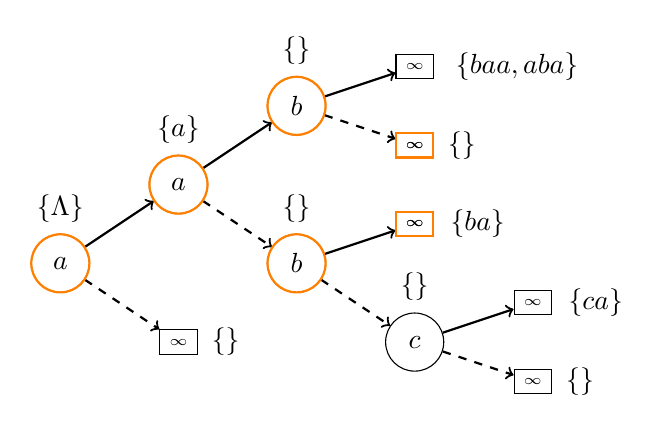
\begin{tikzpicture}
          \tikzstyle{ana_node}       = [shape = circle,    draw = black,         minimum size=21pt]
  \tikzstyle{ana_node__curr} = [shape = circle,    draw = orange, thick, minimum size=21pt]
  \tikzstyle{ana_leaf}       = [shape = rectangle, draw = black,         minimum size=8pt]
  \tikzstyle{ana_leaf__curr} = [shape = rectangle, draw = orange, thick, minimum size=8pt]

  \node[ana_node] at (0.0, 0.0) (n1) {$a$};
  \node           at (0.0, 0.7) {$\{ \Lambda \}$};

  \node[ana_leaf] at (1.5,-1.0) (n1_l1) {\tiny $\infty$};
  \node           at (2.1,-1.0) {$\{\}$};

  \node[ana_node] at (1.5, 1.0) (n2) {$a$};
  \node           at (1.5, 1.7) {$\{ a \}$};

  \node[ana_node] at (3.0, 2.0) (n3) {$b$};
  \node           at (3.0, 2.7) {$\{\}$};

  \node[ana_leaf] at (4.5, 2.5) (n3_l1) {\tiny $\infty$};
  \node           at (5.8, 2.5) {$\{ baa, aba \}$};

  \node[ana_leaf] at (4.5, 1.5) (n3_l2) {\tiny $\infty$};
  \node           at (5.1, 1.5) {$\{\}$};

  \node[ana_node] at (3.0, 0.0) (n4) {$b$};
  \node           at (3.0, 0.7) {$\{\}$};

  \node[ana_leaf] at (4.5, 0.5) (n4_l1) {\tiny $\infty$};
  \node           at (5.3, 0.5) {$\{ ba \}$};

  \node[ana_node] at (4.5,-1.0) (n5) {$c$};
  \node           at (4.5,-0.3) {$\{\}$};

  \node[ana_leaf] at (6.0,-0.5) (n5_l1) {\tiny $\infty$};
  \node           at (6.8,-0.5) {$\{ ca \}$};

  \node[ana_leaf] at (6.0,-1.5) (n5_l2) {\tiny $\infty$};
  \node           at (6.6,-1.5) {$\{\}$};

  \draw[->, solid, thick]
    (n1) edge    (n2)
    (n2) edge (n3)
    (n3) edge (n3_l1)
    (n4) edge (n4_l1)
    (n5) edge (n5_l1)
  ;

  \draw[->, dashed, thick]
    (n1) edge (n1_l1)
    (n2) edge (n4)
    (n3) edge (n3_l2)
    (n4) edge (n5)
    (n5) edge (n5_l2)
  ;


        % n1
        \onslide<3,9>   { \node[ana_node__curr] at (0.0, 0.0) {}; }
        % n2
        \onslide<4,10>  { \node[ana_node__curr] at (1.5, 1.0) {}; }
        % n3
        \onslide<11>    { \node[ana_node__curr] at (3.0, 2.0) {}; }
        % n3_l2
        \onslide<12-13> { \node[ana_leaf__curr] at (4.5, 1.5) {\tiny $\infty$}; }
        % n4
        \onslide<5>     { \node[ana_node__curr] at (3.0, 0.0) {}; }
        % n4_l1
        \onslide<6-7>   { \node[ana_leaf__curr] at (4.5, 0.5) {\tiny $\infty$}; }
      \end{tikzpicture}

      $L = \{ \Lambda, a, ba, ca, aba, baa \}$
    \end{column}
    \begin{column}{0.45\textwidth}
      \small\tt

      \onslide<2->{
        contains(x):\\
        \quad n  := find(root, sort(x), 0)\\
        \quad return n $\neq$ NIL \& n.contains(x)
      }

      \vspace{10pt}

      \onslide<2->{
        find(n, x', i):\\
        \onslide<6->{{\only<6>{\color{orange}}
          \quad if i = x'.length\\
          \qquad return n\\
        }}
        \onslide<12->{{\only<12>{\color{orange}}
          \quad if x'[i] < n.char\\
          \qquad return NIL\\
        }}
        \onslide<4->{{\only<4,11>{\color{orange}}
          \quad if x'[i] > n.char\\
          \qquad return find(n.false, x', i)\\
        }}
        \onslide<3->{{\only<3,5,9-10>{\color{orange}}
          \quad if x'[i] = n.char\\
          \qquad return find(n.true , x', i+1)
        }}
      }
    \end{column}
  \end{columns}
\end{frame}

\begin{frame}
  \frametitle{Anatree.\texttt{contains(\dots)}}

  \begin{columns}
    \begin{column}{0.55\textwidth}
      \centering

      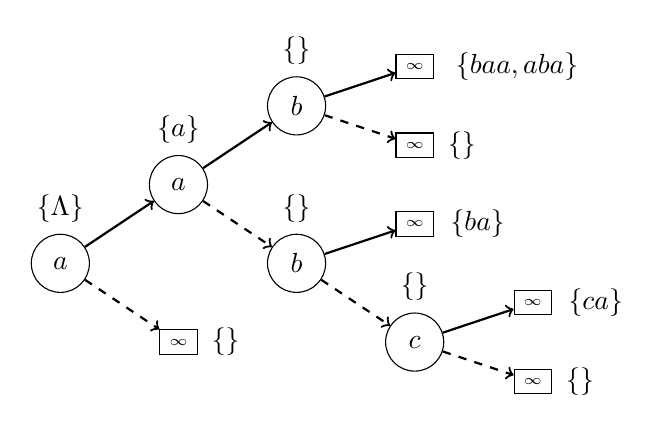
\begin{tikzpicture}
          \tikzstyle{ana_node}       = [shape = circle,    draw = black,         minimum size=21pt]
  \tikzstyle{ana_node__curr} = [shape = circle,    draw = orange, thick, minimum size=21pt]
  \tikzstyle{ana_leaf}       = [shape = rectangle, draw = black,         minimum size=8pt]
  \tikzstyle{ana_leaf__curr} = [shape = rectangle, draw = orange, thick, minimum size=8pt]

  \node[ana_node] at (0.0, 0.0) (n1) {$a$};
  \node           at (0.0, 0.7) {$\{ \Lambda \}$};

  \node[ana_leaf] at (1.5,-1.0) (n1_l1) {\tiny $\infty$};
  \node           at (2.1,-1.0) {$\{\}$};

  \node[ana_node] at (1.5, 1.0) (n2) {$a$};
  \node           at (1.5, 1.7) {$\{ a \}$};

  \node[ana_node] at (3.0, 2.0) (n3) {$b$};
  \node           at (3.0, 2.7) {$\{\}$};

  \node[ana_leaf] at (4.5, 2.5) (n3_l1) {\tiny $\infty$};
  \node           at (5.8, 2.5) {$\{ baa, aba \}$};

  \node[ana_leaf] at (4.5, 1.5) (n3_l2) {\tiny $\infty$};
  \node           at (5.1, 1.5) {$\{\}$};

  \node[ana_node] at (3.0, 0.0) (n4) {$b$};
  \node           at (3.0, 0.7) {$\{\}$};

  \node[ana_leaf] at (4.5, 0.5) (n4_l1) {\tiny $\infty$};
  \node           at (5.3, 0.5) {$\{ ba \}$};

  \node[ana_node] at (4.5,-1.0) (n5) {$c$};
  \node           at (4.5,-0.3) {$\{\}$};

  \node[ana_leaf] at (6.0,-0.5) (n5_l1) {\tiny $\infty$};
  \node           at (6.8,-0.5) {$\{ ca \}$};

  \node[ana_leaf] at (6.0,-1.5) (n5_l2) {\tiny $\infty$};
  \node           at (6.6,-1.5) {$\{\}$};

  \draw[->, solid, thick]
    (n1) edge    (n2)
    (n2) edge (n3)
    (n3) edge (n3_l1)
    (n4) edge (n4_l1)
    (n5) edge (n5_l1)
  ;

  \draw[->, dashed, thick]
    (n1) edge (n1_l1)
    (n2) edge (n4)
    (n3) edge (n3_l2)
    (n4) edge (n5)
    (n5) edge (n5_l2)
  ;

      \end{tikzpicture}

      $L = \{ \Lambda, a, ba, ca, aba, baa \}$
    \end{column}
    \begin{column}{0.45\textwidth}
      \begin{lemma}
        \texttt{find(n, sort(x), i)} runs in\\$\Oh{\sort{\abs{x}} + \abs{\Sigma}}$ time.
      \end{lemma}
      \begin{proof}
        $\Oh{1}$ time is spent per node\only<1>{. At most
          $\abs{x}$ \emph{high} edges and
          $\abs{\Sigma}$ \emph{low} edges are traversed, meaning at most $\abs{x} +
          \abs{\Sigma}$ nodes are visited.

          On top of this, add the $\Oh{\sort{\abs{x}}}$ time to sort $x$ into $x'$.
        }%
        \only<2->{\dots}
      \end{proof}

      \only<2>{
        \vspace{32.5pt}

        \begin{corollary}
          \texttt{contains(x)} runs in\\$\Oh{\sort{\abs{x}} + \abs{\Sigma}}$ time.
        \end{corollary}
      }
    \end{column}
  \end{columns}
\end{frame}


\subsection{\texttt{anagrams(x)}}

\begin{frame}[fragile]
  \frametitle{Anatree.\texttt{anagrams(\dots)}}

  \begin{columns}
    \begin{column}{0.55\textwidth}
      \centering

      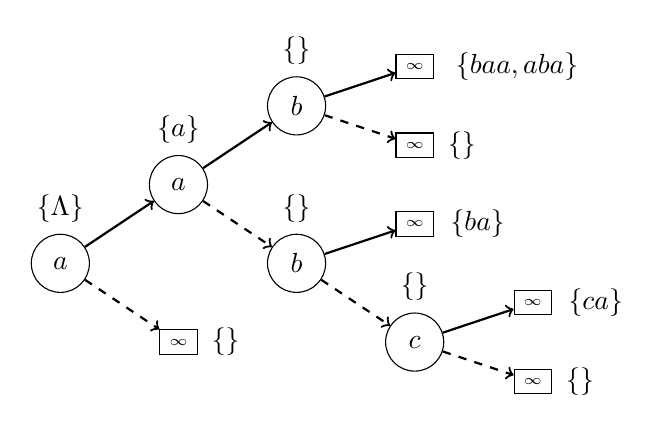
\begin{tikzpicture}
          \tikzstyle{ana_node}       = [shape = circle,    draw = black,         minimum size=21pt]
  \tikzstyle{ana_node__curr} = [shape = circle,    draw = orange, thick, minimum size=21pt]
  \tikzstyle{ana_leaf}       = [shape = rectangle, draw = black,         minimum size=8pt]
  \tikzstyle{ana_leaf__curr} = [shape = rectangle, draw = orange, thick, minimum size=8pt]

  \node[ana_node] at (0.0, 0.0) (n1) {$a$};
  \node           at (0.0, 0.7) {$\{ \Lambda \}$};

  \node[ana_leaf] at (1.5,-1.0) (n1_l1) {\tiny $\infty$};
  \node           at (2.1,-1.0) {$\{\}$};

  \node[ana_node] at (1.5, 1.0) (n2) {$a$};
  \node           at (1.5, 1.7) {$\{ a \}$};

  \node[ana_node] at (3.0, 2.0) (n3) {$b$};
  \node           at (3.0, 2.7) {$\{\}$};

  \node[ana_leaf] at (4.5, 2.5) (n3_l1) {\tiny $\infty$};
  \node           at (5.8, 2.5) {$\{ baa, aba \}$};

  \node[ana_leaf] at (4.5, 1.5) (n3_l2) {\tiny $\infty$};
  \node           at (5.1, 1.5) {$\{\}$};

  \node[ana_node] at (3.0, 0.0) (n4) {$b$};
  \node           at (3.0, 0.7) {$\{\}$};

  \node[ana_leaf] at (4.5, 0.5) (n4_l1) {\tiny $\infty$};
  \node           at (5.3, 0.5) {$\{ ba \}$};

  \node[ana_node] at (4.5,-1.0) (n5) {$c$};
  \node           at (4.5,-0.3) {$\{\}$};

  \node[ana_leaf] at (6.0,-0.5) (n5_l1) {\tiny $\infty$};
  \node           at (6.8,-0.5) {$\{ ca \}$};

  \node[ana_leaf] at (6.0,-1.5) (n5_l2) {\tiny $\infty$};
  \node           at (6.6,-1.5) {$\{\}$};

  \draw[->, solid, thick]
    (n1) edge    (n2)
    (n2) edge (n3)
    (n3) edge (n3_l1)
    (n4) edge (n4_l1)
    (n5) edge (n5_l1)
  ;

  \draw[->, dashed, thick]
    (n1) edge (n1_l1)
    (n2) edge (n4)
    (n3) edge (n3_l2)
    (n4) edge (n5)
    (n5) edge (n5_l2)
  ;

      \end{tikzpicture}

      $L = \{ \Lambda, a, ba, ca, aba, baa \}$
    \end{column}
    \begin{column}{0.45\textwidth}
      \small\tt

      anagrams(x):\\
      \quad n  := find(root, sort(x), 0)\\
      \quad if n $\neq$ NIL\\
      \qquad output words in n

      \vspace{10pt}

      \begin{corollary}
        \texttt{anagrams(x)} runs in\\$\Oh{\sort{\abs{x}} + \abs{\Sigma} + T}$ time.
      \end{corollary}
      \begin{proof}
        It takes $\Oh{\sort{\abs{x}} + \abs{\Sigma}}$ time to find
        $n$ and then another $\Oh{T}$ time to output its content.
      \end{proof}
    \end{column}
  \end{columns}
\end{frame}

\subsection{\texttt{subanagrams(x)}}

\begin{frame}
  \frametitle{Anatree.\texttt{subanagrams(\only<-6>{a}\only<7->{abb})
      = \only<2-6,8->{$\Lambda$}\only<5-6,10->{, a}\only<14-15>{, ab}}}

  \begin{columns}
    \begin{column}{0.55\textwidth}
      \centering

      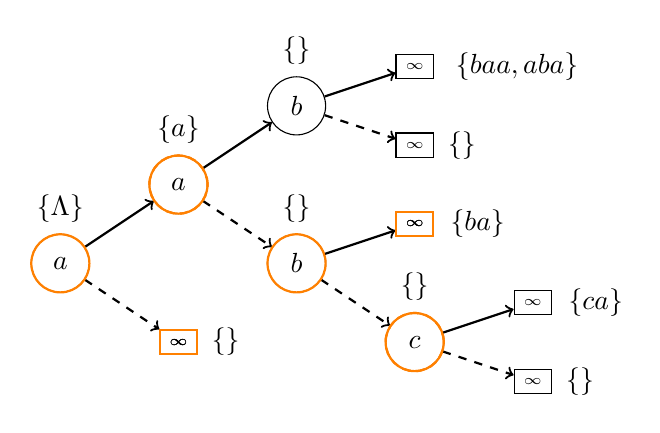
\begin{tikzpicture}
          \tikzstyle{ana_node}       = [shape = circle,    draw = black,         minimum size=21pt]
  \tikzstyle{ana_node__curr} = [shape = circle,    draw = orange, thick, minimum size=21pt]
  \tikzstyle{ana_leaf}       = [shape = rectangle, draw = black,         minimum size=8pt]
  \tikzstyle{ana_leaf__curr} = [shape = rectangle, draw = orange, thick, minimum size=8pt]

  \node[ana_node] at (0.0, 0.0) (n1) {$a$};
  \node           at (0.0, 0.7) {$\{ \Lambda \}$};

  \node[ana_leaf] at (1.5,-1.0) (n1_l1) {\tiny $\infty$};
  \node           at (2.1,-1.0) {$\{\}$};

  \node[ana_node] at (1.5, 1.0) (n2) {$a$};
  \node           at (1.5, 1.7) {$\{ a \}$};

  \node[ana_node] at (3.0, 2.0) (n3) {$b$};
  \node           at (3.0, 2.7) {$\{\}$};

  \node[ana_leaf] at (4.5, 2.5) (n3_l1) {\tiny $\infty$};
  \node           at (5.8, 2.5) {$\{ baa, aba \}$};

  \node[ana_leaf] at (4.5, 1.5) (n3_l2) {\tiny $\infty$};
  \node           at (5.1, 1.5) {$\{\}$};

  \node[ana_node] at (3.0, 0.0) (n4) {$b$};
  \node           at (3.0, 0.7) {$\{\}$};

  \node[ana_leaf] at (4.5, 0.5) (n4_l1) {\tiny $\infty$};
  \node           at (5.3, 0.5) {$\{ ba \}$};

  \node[ana_node] at (4.5,-1.0) (n5) {$c$};
  \node           at (4.5,-0.3) {$\{\}$};

  \node[ana_leaf] at (6.0,-0.5) (n5_l1) {\tiny $\infty$};
  \node           at (6.8,-0.5) {$\{ ca \}$};

  \node[ana_leaf] at (6.0,-1.5) (n5_l2) {\tiny $\infty$};
  \node           at (6.6,-1.5) {$\{\}$};

  \draw[->, solid, thick]
    (n1) edge    (n2)
    (n2) edge (n3)
    (n3) edge (n3_l1)
    (n4) edge (n4_l1)
    (n5) edge (n5_l1)
  ;

  \draw[->, dashed, thick]
    (n1) edge (n1_l1)
    (n2) edge (n4)
    (n3) edge (n3_l2)
    (n4) edge (n5)
    (n5) edge (n5_l2)
  ;


        % n1
        \onslide<2-3,8>   { \node[ana_node__curr] at (0.0, 0.0) {}; }

        % n1_l1
        \onslide<3,8>     { \node[ana_leaf__curr, densely dashed] at (1.5,-1.0) {\tiny $\infty$}; }
        \onslide<4,9>     { \node[ana_leaf__curr] at (1.5,-1.0) {\tiny $\infty$}; }

        % n2
        \onslide<3-4,8-9> { \node[ana_node__curr, densely dashed] at (1.5, 1.0) {}; }
        \onslide<5,10>    { \node[ana_node__curr] at (1.5, 1.0) {}; }

        % n4
        \onslide<11>      { \node[ana_node__curr] at (3.0, 0.0) {}; }

        % n4_l1
        \onslide<11-13>   { \node[ana_leaf__curr, densely dashed] at (4.5, 0.5) (n4_l1) {\tiny $\infty$}; }
        \onslide<14>      { \node[ana_leaf__curr] at (4.5, 0.5) (n4_l1) {\tiny $\infty$}; }

        % n5
        \onslide<11>      { \node[ana_node__curr, densely dashed] at (4.5,-1.0) {}; }
        \onslide<12-13>   { \node[ana_node__curr] at (4.5,-1.0) {}; }
      \end{tikzpicture}

      $L = \{ \Lambda, a, ba, ca, aba, baa \}$
    \end{column}
    \begin{column}{0.45\textwidth}
      \footnotesize\tt

      subanagrams(x):\\
      \quad subanagrams'(root, sort(x), 0)\\

      \vspace{6pt}

      \onslide<2->{
        subanagrams'(n, x', i):\\
        \onslide<2->{{\only<2>{\color{orange}}
          \quad output words in n\\
        }}
        \onslide<4->{{\only<4,9,14>{\color{orange}}
          \quad if n.char = $\infty$:\\
          \qquad return\\
        }}
        \onslide<12->{{\only<12>{\color{orange}}
          \quad while x'[i] < n.char:\\
          \qquad i++\\
        }}
        \onslide<5->{{\only<5,13>{\color{orange}}
          \quad if i = x'.length:\\
          \qquad return\\
        }}
        \onslide<10->{{\only<10>{\color{orange}}
          \quad if x'[i] > n.char:\\
          \qquad subanagrams'(n.false, x', i)\\
        }}
        \onslide<3->{{\only<3,8,11>{\color{orange}}
            \quad if x'[i] = n.char:\\
            \qquad subanagrams'(n.false, x', i+1)\\
            \qquad subanagrams'(n.true,\phantom{n} x', i+1)\\
        }}
      }
    \end{column}
  \end{columns}
\end{frame}

\begin{frame}
  \frametitle{Anatree.\texttt{subanagrams(\dots)}}

  \begin{columns}
    \begin{column}{0.55\textwidth}
      \centering

      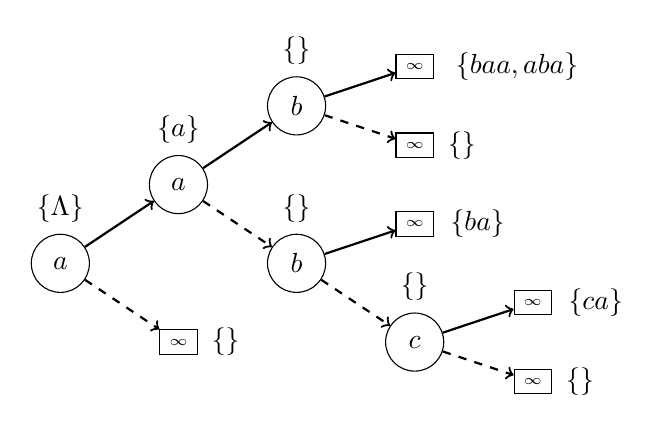
\begin{tikzpicture}
          \tikzstyle{ana_node}       = [shape = circle,    draw = black,         minimum size=21pt]
  \tikzstyle{ana_node__curr} = [shape = circle,    draw = orange, thick, minimum size=21pt]
  \tikzstyle{ana_leaf}       = [shape = rectangle, draw = black,         minimum size=8pt]
  \tikzstyle{ana_leaf__curr} = [shape = rectangle, draw = orange, thick, minimum size=8pt]

  \node[ana_node] at (0.0, 0.0) (n1) {$a$};
  \node           at (0.0, 0.7) {$\{ \Lambda \}$};

  \node[ana_leaf] at (1.5,-1.0) (n1_l1) {\tiny $\infty$};
  \node           at (2.1,-1.0) {$\{\}$};

  \node[ana_node] at (1.5, 1.0) (n2) {$a$};
  \node           at (1.5, 1.7) {$\{ a \}$};

  \node[ana_node] at (3.0, 2.0) (n3) {$b$};
  \node           at (3.0, 2.7) {$\{\}$};

  \node[ana_leaf] at (4.5, 2.5) (n3_l1) {\tiny $\infty$};
  \node           at (5.8, 2.5) {$\{ baa, aba \}$};

  \node[ana_leaf] at (4.5, 1.5) (n3_l2) {\tiny $\infty$};
  \node           at (5.1, 1.5) {$\{\}$};

  \node[ana_node] at (3.0, 0.0) (n4) {$b$};
  \node           at (3.0, 0.7) {$\{\}$};

  \node[ana_leaf] at (4.5, 0.5) (n4_l1) {\tiny $\infty$};
  \node           at (5.3, 0.5) {$\{ ba \}$};

  \node[ana_node] at (4.5,-1.0) (n5) {$c$};
  \node           at (4.5,-0.3) {$\{\}$};

  \node[ana_leaf] at (6.0,-0.5) (n5_l1) {\tiny $\infty$};
  \node           at (6.8,-0.5) {$\{ ca \}$};

  \node[ana_leaf] at (6.0,-1.5) (n5_l2) {\tiny $\infty$};
  \node           at (6.6,-1.5) {$\{\}$};

  \draw[->, solid, thick]
    (n1) edge    (n2)
    (n2) edge (n3)
    (n3) edge (n3_l1)
    (n4) edge (n4_l1)
    (n5) edge (n5_l1)
  ;

  \draw[->, dashed, thick]
    (n1) edge (n1_l1)
    (n2) edge (n4)
    (n3) edge (n3_l2)
    (n4) edge (n5)
    (n5) edge (n5_l2)
  ;

      \end{tikzpicture}

      $L = \{ \Lambda, a, ba, ca, aba, baa \}$
    \end{column}
    \begin{column}{0.45\textwidth}
      \small

      \begin{lemma}
        For $N = \sum_{i = 1}^k \abs{x_i}$, the anatree has size, $N_{\text{tree}}$, at most $N$.
      \end{lemma}

      \pause

      \begin{theorem}
        \texttt{subanagrams(x)} runs in\\
        $\Oh{\sort{\abs{x}} + \min(N_{\text{tree}}, 2^{\abs{x}} \cdot \abs{\Sigma}) + T}$ time.
      \end{theorem}
      \begin{proof}
        It takes $\Oh{\sort{\abs{x}}}$ time to sort $x$ and another $\Oh{T}$ to write the output.

        For every match, the recursion splits in two. Each of these
        $2^{\abs{x}}$ matches have $\abs{\Sigma}$ or fewer mismatches.
      \end{proof}
    \end{column}
  \end{columns}
\end{frame}

\begin{frame}
  \frametitle{Anatree.\texttt{keys(\dots)}}

  \begin{definition}
    The subset $L'$ of $L \subseteq \Sigma^*$ is a set of keys w.r.t.\ $\Psi$ if for all
    $x, y \in L'$ then $\Psi(x) \neq \Psi(y)$.
  \end{definition}

  \vspace{30pt}
  \pause

  \centering
  \begin{minipage}{.74\textwidth\relax}
    \large

    \begin{theorem}
      \texttt{keys(length)} runs in $\Oh{\min(N_{\text{tree}}, 2^{\texttt{length}} \cdot \abs{\Sigma}) + T}$ time.
    \end{theorem}
    \begin{proof}
      Left as an exercise to the reader\dots
    \end{proof}

  \end{minipage}
\end{frame}

\subsection{\texttt{insert(x)}}

\begin{frame}
  \frametitle{Anatree.\texttt{insert(%
      \only<1-2>{$\Lambda$}%
      \only<3-6>{$ba$}%
      \only<7-9>{$a$}%
      \only<10-17>{$baa$}%
      \only<18-22>{$aba$}%
      \only<23-28>{$ca$}%
      \only<29->{\dots}%
      )}}

  \begin{columns}
    \begin{column}{0.48\textwidth}
      \centering

      \begin{tikzpicture}
        \tikzstyle{ana_node}       = [shape = circle,    draw = black,         minimum size=21pt]
        \tikzstyle{ana_node__curr} = [shape = circle,    draw = orange, thick, minimum size=21pt]
        \tikzstyle{ana_leaf}       = [shape = rectangle, draw = black,         minimum size=8pt]
        \tikzstyle{ana_leaf__curr} = [shape = rectangle, draw = orange, thick, minimum size=8pt]

        % n1
        \onslide<1-3> {
          \node[ana_leaf]       at (0.0, 0.0) (r_l) {\tiny $\infty$};
        }
        \only<2>{
          \node[ana_leaf__curr] at (0.0, 0.0) (n1) {\tiny $\infty$};
        }

        \onslide<4-> {
          \node[ana_node]       at (0.0, 0.0) (n1) {a};
        }
        \only<4,8,11,19,24> {
          \node[ana_node__curr] at (0.0, 0.0) {};
        }

        \only<1> {
          \node at (0.0, 0.7) {$\{ \}$};
        }
        \onslide<2-> {
          \node at (0.0, 0.7) {$\{ \Lambda \}$};
        }

        % n1_l1
        \onslide<4-> {
          \node[ana_leaf]       at (1.2,-1.0) (n1_l1) {\tiny $\infty$};
          \node                 at (1.8,-1.0) {$\{\}$};

          \draw[->, dashed, thick] (n1) edge (n1_l1);
        }

        % n2
        \onslide<13-> {
          \node[ana_node]       at (1.3, 1.0) (n2) {$a$};
          \node                 at (1.3, 1.7) {$\{ \only<14->{a} \}$};
        }
        \onslide<15-> {
          \draw[->, thick] (n1) edge (n2);
        }
        \only<13-15,20,25> {
          \node[ana_node__curr] at (1.3, 1.0) {};
        }

        % n3
        \onslide<13-15> {
          \node[ana_leaf]       at (2.4, 2.0) (n3_l) {\tiny $\infty$};
          \draw[->, thick] (n2) edge (n3_l);
        }
        \onslide<16-> {
          \node[ana_node]       at (2.4, 2.0) (n3) {$b$};
          \draw[->, thick] (n2) edge (n3);
        }
        \only<16,21> {
          \node[ana_node__curr] at (2.4, 2.0) {};
        }
        \onslide<13-> {
          \node                 at (2.4, 2.7) {$\{\}$};
        }

        % n3_l1
        \onslide<16-> {
          \node[ana_leaf]       at (3.6, 2.5) (n3_l1) {\tiny $\infty$};
          \draw[->, thick] (n3) edge (n3_l1);
        }
        \onslide<17,22> {
          \node[ana_leaf__curr] at (3.6, 2.5) {\tiny $\infty$};
        }
        \onslide<16> {
          \node                 at (4.2, 2.5) {$\{ \}$};
        }
        \onslide<17-21>{
          \node                 at (4.5, 2.5) {$\{ baa \}$};
        }
        \onslide<22-> {
          \node                 at (4.86, 2.5) {$\{ baa, aba \}$};
        }

        % n3_l2
        \onslide<16-> {
          \node[ana_leaf]       at (3.6, 1.5) (n3_l2) {\tiny $\infty$};
          \node                 at (4.2, 1.5) {$\{\}$};
          \draw[->, dashed, thick] (n3) edge (n3_l2);
        }

        % n4
        \only<4> {
          \node[ana_leaf]       at (2.4, 0.0) (n4_l) {\tiny $\infty$};
          \draw[->, thick] (n1) edge (n4_l);
        }
        \onslide<5-> {
          \node[ana_node]       at (2.4, 0.0) (n4) {$b$};
        }
        \onslide<5-14> {
          \draw[->, thick] (n1) edge (n4);
        }
        \onslide<13-> {
          \draw[->, dashed, thick] (n2) edge (n4);
        }
        \onslide<4-> {
          \node                 at (2.4, 0.7) {$\{ \only<9-13>{a} \}$};
        }
        \only<5,9,12,26> {
          \node[ana_node__curr] at (2.4, 0.0) {};
        }
        \only<13-15>  {
          \node[ana_node__curr, densely dashed] at (2.4, 0.0) {};
        }

        % n4_l1
        \onslide<5-> {
          \node[ana_leaf]       at (3.6, 0.5) (n4_l1) {\tiny $\infty$};
          \draw[->, thick] (n4) edge (n4_l1);
        }
        \only<5> {
          \node                 at (4.2, 0.5) {$\{ \}$};
        }
        \onslide<6-> {
          \node                 at (4.4, 0.5) {$\{ ba \}$};
        }
        \only<6> {
          \node[ana_leaf__curr] at (3.6, 0.5) {\tiny $\infty$};
        }

        % n5
        \onslide<5-26> {
          \node[ana_leaf]       at (3.6,-1.0) (n5_l) {\tiny $\infty$};
          \draw[->, dashed, thick] (n4) edge (n5_l);
        }
        \onslide<5-> {
          \node                 at (3.6,-0.3) {$\{\}$};
        }
        \onslide<27-> {
          \node[ana_node]       at (3.6,-1.0) (n5) {$c$};
          \draw[->, dashed, thick] (n4) edge (n5);
        }
        \only<27> {
          \node[ana_node__curr] at (3.6,-1.0) {};
        }

        % n5_l1
        \onslide<27-> {
          \node[ana_leaf]       at (4.8,-0.5) (n5_l1) {\tiny $\infty$};
          \draw[->, thick] (n5) edge (n5_l1);
        }
        \onslide<27> {
          \node                 at (5.4,-0.5) {$\{\}$};
        }
        \onslide<28-> {
          \node                 at (5.6,-0.5) {$\{ ca \}$};
        }
        \only<28> {
          \node[ana_leaf__curr] at (4.8,-0.5) {\tiny $\infty$};
        }

        % n5_l2
        \onslide<27-> {
          \node[ana_leaf]       at (4.8,-1.5) (n5_l2) {\tiny $\infty$};
          \node                 at (5.4,-1.5) {$\{\}$};
          \draw[->, dashed, thick] (n5) edge (n5_l2);
        }
      \end{tikzpicture}

      % NOTE: $\Lambda$, ba, a, baa, aba, c, ca,
    \end{column}
    \begin{column}{0.52\textwidth}
      \scriptsize\tt

      insert(x):\\
      \quad root = insert'(root, sort(x), 0, x)\\

      \vspace{6pt}

      insert'(n, x', i, x):\\
      \onslide<2-> {{\only<2,6,9,17,22,28>{\color{orange}}
        \quad if i = x'.length:\\
        \qquad n.insert(x)\\
      }}
      \onslide<4-> {{\only<4,5,16,27>{\color{orange}}
        \quad else if n.char = $\infty$:\\
        \qquad n = node\{ char:\ x'[i], false:\ $\infty$, true:\ $\infty$ \}\\
        \qquad n.true = insert'(n.true, x', i+1, x)\\
      }}
      \onslide<12-> {{\only<12-15>{\color{orange}}
        \quad else if x'[i] < m.char:\\
        \qquad n' = node\{ char:\ x'[i], false:\ n, true:\ $\infty$ \}\\
        \qquad move n.words into n'.words\\
        \qquad n'.true = insert'(n'.true, x', i+1, x)\\
        \qquad return n'\\
      }}
      \onslide<25-> {{\only<25-26>{\color{orange}}
      \quad else if x'[i] > m.char:\\
      \qquad n.false = insert'(n.false, x', i, x)\\
      }}
      \onslide<8-> {{\only<8,11,19-21,24>{\color{orange}}
        \quad else if x'[i] == m.char:\\
        \qquad n.true = insert'(n.true, x', i+1, x)\\
      }}
      \onslide<2-> {{\only<2,4-6,8-9,11,16-17,19-22,24-28>{\color{orange}}
        \quad return n\\
      }}
    \end{column}
  \end{columns}
\end{frame}

\begin{frame}
  \frametitle{Anatree.\texttt{insert(\dots)}}

  \begin{theorem}
    \texttt{insert($x$)} runs in $\Oh{\sort{\abs{x}} + \Sigma}$ time.
  \end{theorem}
  \begin{proof}
    Similar argument as for \texttt{find($n$, $x'$, $i$)}.
  \end{proof}

  \pause

  \begin{corollary}
    For $N = \sum_{i = 1}^k \abs{x_i}$, \texttt{insert($x_1$, $x_2$, \dots, $x_k$)} requires
    $\Oh{\sort{N} + k \cdot \abs{\Sigma}}$ time.
  \end{corollary}
  \begin{proof}
    Follows from complexity of \texttt{insert($x_i$)} and \texttt{sort} distributes over $+$ in
    $\mathcal{O}$-notation:

    \qquad $\Oh{\sort{N_1} + \sort{N_2}} = \Oh{\sort{N_1 + N_2}}$
  \end{proof}
\end{frame}

\begin{frame}
  \frametitle{Anatree.\texttt{delete(\dots)}}

  \centering
  \begin{minipage}{.63\textwidth\relax}
    \Large

  \begin{theorem}
    \texttt{delete($x$)} runs in $\Oh{\sort{\abs{x}} + \abs{\Sigma}}$ time.
  \end{theorem}
  \begin{proof}
    Left as an exercise to the reader\dots
  \end{proof}

  \end{minipage}
\end{frame}

% ------------------------------------------------------------------------------------------------ %
\blankframe
% ------------------------------------------------------------------------------------------------ %

\flagsdefault[width=9pt, framewidth=0.1pt]

\begin{frame}
  \frametitle{Anatree}

  \begin{table}
    \centering
    \begin{tabular}{cl|cc|rrrr}
                     &    & \multicolumn{2}{c|}{Dictionary} & \multicolumn{4}{c}{Anatree}
      \\
                     &    &  \small \# Words
                                     & \small \# Symbols
                                                            & \small Size
                                                                    & \small {\#}Keys
                                                                               & \small \texttt{insert} (s)
                                                                                       & \small\texttt{subanagrams} (s)
      \\ \hline \hline
      \worldflag{DK} & DK & 32863    & 177308               & 62687 & 8513     & 12.62 & 1.05
      \\
      \worldflag{DE} & DE & 23587    & 127562               & 55047 & 8201     &  9.46 & 0.88
      \\
      \worldflag{GB} & EN & 40804    & 218342               & 75697 & 11741    & 10.62 & 1.43
      \\
      \worldflag{ES} & ES & 39650    & 219776               & 56103 & 7502     &  8.45 & 0.89
    \end{tabular}
  \end{table}
\end{frame}

% ------------------------------------------------------------------------------------------------ %
% ------------------------------------------------------------------------------------------------ %

\section{Multi-valued Anatree}

\begin{frame}[plain,noframenumbering]{}
  \frametitle{Contents}
  \tableofcontents[currentsection]
\end{frame}

\begin{frame}
  \frametitle{Multi-valued Anatree}

  \centering

  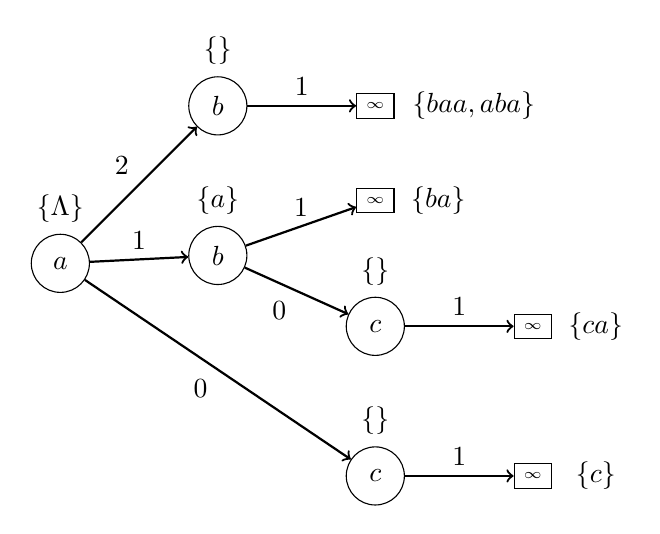
\begin{tikzpicture}
    \tikzstyle{ana_node}       = [shape = circle,    draw = black,         minimum size=21pt]
    \tikzstyle{ana_node__curr} = [shape = circle,    draw = orange, thick, minimum size=21pt]
    \tikzstyle{ana_leaf}       = [shape = rectangle, draw = black,         minimum size=8pt]
    \tikzstyle{ana_leaf__curr} = [shape = rectangle, draw = orange, thick, minimum size=8pt]

    \node[ana_node] at (0.0,  0.0) (n1) {$a$};
    \node           at (0.0,  0.7) {$\{ \Lambda \}$};

    \node[ana_node] at (2.0,  2.0) (n3) {$b$};
    \node           at (2.0,  2.7) {$\{\}$};

    \node[ana_leaf] at (4.0,  2.0) (n3_l1) {\tiny $\infty$};
    \node           at (5.25, 2.0) {$\{ baa, aba \}$};

    \node[ana_node] at (2.0,  0.1) (n4) {$b$};
    \node           at (2.0,  0.8) {$\{ a \}$};

    \node[ana_leaf] at (4.0,  0.8) (n4_l1) {\tiny $\infty$};
    \node           at (4.8,  0.8) {$\{ ba \}$};

    \node[ana_node] at (4.0, -0.8) (n5) {$c$};
    \node           at (4.0, -0.1) {$\{\}$};

    \node[ana_leaf] at (6.0, -0.8) (n5_l1) {\tiny $\infty$};
    \node           at (6.8, -0.8) {$\{ ca \}$};

    \node[ana_node] at (4.0, -2.7) (n6) {$c$};
    \node           at (4.0, -2.0) {$\{\}$};

    \node[ana_leaf] at (6.0, -2.7) (n6_l1) {\tiny $\infty$};
    \node           at (6.8, -2.7) {$\{ c \}$};

    \draw[->, solid, thick]
      (n1) edge node[above left] {2} (n3)
      (n1) edge node[above] {1} (n4)
      (n3) edge node[above] {1} (n3_l1)
      (n4) edge node[above] {1} (n4_l1)
      (n4) edge node[below left] {0} (n5)
      (n5) edge node[above] {1} (n5_l1)
      (n1) edge node[below left] {0} (n6)
      (n6) edge node[above] {1} (n6_l1)
    ;
  \end{tikzpicture}

  $L = \{ \Lambda, a, c, ba, ca, aba, baa \}$
\end{frame}

% ------------------------------------------------------------------------------------------------ %
% ------------------------------------------------------------------------------------------------ %

\section{Letter Ordering}

\begin{frame}[plain,noframenumbering]{}
  \frametitle{Contents}
  \tableofcontents[currentsection]
\end{frame}

\begin{frame}
  \frametitle{Letter Ordering}

  \begin{columns}
    \begin{column}{0.5\textwidth}
      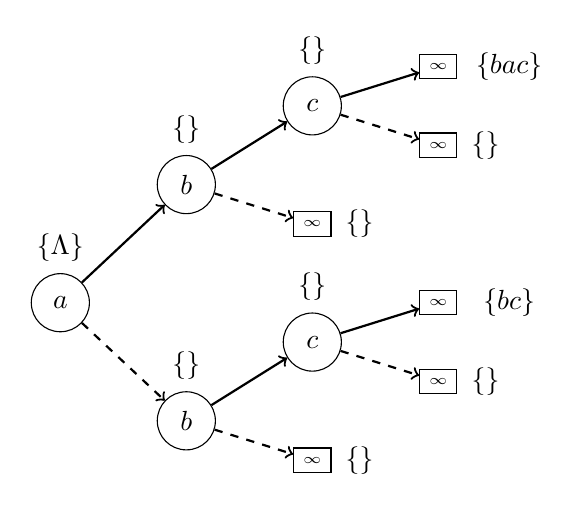
\begin{tikzpicture}
        \tikzstyle{ana_node}       = [shape = circle,    draw = black,         minimum size=21pt]
        \tikzstyle{ana_leaf}       = [shape = rectangle, draw = black,         minimum size=8pt]

        \node[ana_node] at (0.0,  0.0) (n1) {$a$};
        \node           at (0.0,  0.7) {$\{ \Lambda \}$};

        \node[ana_node] at (1.6,  1.5) (n2) {$b$};
        \node           at (1.6,  2.2) {$\{\}$};

        \node[ana_leaf] at (3.2,  1.0) (n2_l1) {\tiny $\infty$};
        \node           at (3.8,  1.0) {$\{\}$};

        \node[ana_node] at (3.2,  2.5) (n3) {$c$};
        \node           at (3.2,  3.2) {$\{\}$};

        \node[ana_leaf] at (4.8,  3.0) (n3_l1) {\tiny $\infty$};
        \node           at (5.7,  3.0) {$\{ bac \}$};

        \node[ana_leaf] at (4.8,  2.0) (n3_l2) {\tiny $\infty$};
        \node           at (5.4,  2.0) {$\{\}$};

        \node[ana_node] at (1.6, -1.5) (n4) {$b$};
        \node           at (1.6, -0.8) {$\{\}$};

        \node[ana_leaf] at (3.2, -2.0) (n4_l1) {\tiny $\infty$};
        \node           at (3.8, -2.0) {$\{ \}$};

        \node[ana_node] at (3.2, -0.5) (n5) {$c$};
        \node           at (3.2,  0.2) {$\{\}$};

        \node[ana_leaf] at (4.8,  0.0) (n5_l1) {\tiny $\infty$};
        \node           at (5.7,  0.0) {$\{ bc \}$};

        \node[ana_leaf] at (4.8, -1.0) (n5_l2) {\tiny $\infty$};
        \node           at (5.4, -1.0) {$\{\}$};

        \draw[->, dashed, thick]
          (n1) edge (n4)
          (n2) edge (n2_l1)
          (n3) edge (n3_l2)
          (n4) edge (n4_l1)
          (n5) edge (n5_l2)
        ;

        \draw[->, thick]
          (n1) edge (n2)
          (n2) edge (n3)
          (n3) edge (n3_l1)
          (n4) edge (n5)
          (n5) edge (n5_l1)
        ;
      \end{tikzpicture}
    \end{column}
    \begin{column}{0.5\textwidth}
      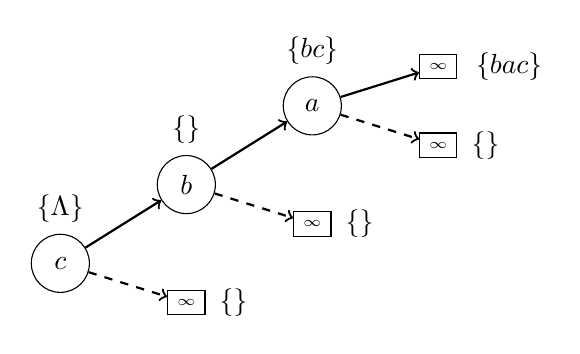
\begin{tikzpicture}
        \tikzstyle{ana_node}       = [shape = circle,    draw = black,         minimum size=21pt]
        \tikzstyle{ana_leaf}       = [shape = rectangle, draw = black,         minimum size=8pt]

        \node[ana_node] at (0.0,  0.0) (n1) {$c$};
        \node           at (0.0,  0.7) {$\{ \Lambda \}$};

        \node[ana_leaf] at (1.6, -0.5) (n1_l1) {\tiny $\infty$};
        \node           at (2.2, -0.5) {$\{\}$};

        \node[ana_node] at (1.6,  1.0) (n2) {$b$};
        \node           at (1.6,  1.7) {$\{\}$};

        \node[ana_leaf] at (3.2,  0.5) (n2_l1) {\tiny $\infty$};
        \node           at (3.8,  0.5) {$\{ \}$};

        \node[ana_node] at (3.2,  2.0) (n3) {$a$};
        \node           at (3.2,  2.7) {$\{ bc \}$};

        \node[ana_leaf] at (4.8,  2.5) (n3_l1) {\tiny $\infty$};
        \node           at (5.7,  2.5) {$\{ bac \}$};

        \node[ana_leaf] at (4.8,  1.5) (n3_l2) {\tiny $\infty$};
        \node           at (5.4,  1.5) {$\{\}$};

        \draw[->, dashed, thick]
          (n1) edge (n1_l1)
          (n2) edge (n2_l1)
          (n3) edge (n3_l2)
        ;

        \draw[->, thick]
          (n1) edge (n2)
          (n2) edge (n3)
          (n3) edge (n3_l1)
        ;
      \end{tikzpicture}
    \end{column}
  \end{columns}

  \centering

  $L = \{ \Lambda, bc, bac \}$
\end{frame}

\iffalse
\begin{frame}
  \frametitle{Letter Ordering}

  \begin{table}
    \centering
    \begin{tabular}{cl|cc|rrrr}
                     &    & \multicolumn{2}{c|}{Dictionary} & \multicolumn{4}{c}{Anatree Size}
      \\
                     &    &  \small \# Words
                                     & \small \# Symbols
                                                            & \small abc...
                                                                    & \small zyx...
                                                                               & \small esi...
                                                                                       & \small qjx...
      \\ \hline \hline
      \worldflag{DK} & DK & 32863    & 177308               & 62687 & 74885    & 57603 & 78849
      \\
      \worldflag{DE} & DE & 23587    & 127562               & 55047 & 64825    & 50409 & 67529
      \\
      \worldflag{GB} & EN & 40804    & 218342               & 75697 & 86185    & 69531 & 91011
      \\
      \worldflag{ES} & ES & 39650    & 219776               & 56103 & 71915    & 50637 & 68383
    \end{tabular}
  \end{table}
\end{frame}
\fi

\begin{frame}
  \frametitle{Letter Ordering}

  \begin{figure}
    \centering

    \begin{tikzpicture}
        \begin{axis}[
          ybar,
          bar width = 0.2,
          % x axis
          xmin=0.3,
          xmax=4.7,
          xticklabel=\empty,
          xtick={1,2,3,4},
          xticklabels={
            \worldflag{DK} DK,
            \worldflag{DE} DE,
            \worldflag{GB} EN,
            \worldflag{ES} ES
          },
          % y axis
          every tick label/.append style={font=\scriptsize},
          ymin=0,
          ymax=100000,
          ylabel={Anatree Size},
          % dimensions
          width=0.9\linewidth,
          height=0.5\linewidth,
          % legend
          legend cell align=left,
          legend pos=north west,
          legend style={draw=black,fill=white},
          legend columns=4
          ]

          % --------------------------------------------------
          % ABC...
          \addplot[draw=black] coordinates {
            (1, 62687)
            (2, 55047)
            (3, 75697)
            (4, 56103)
          };

          % --------------------------------------------------
          % ZYX...
          \addplot[draw=black, pattern=north east lines] coordinates {
            (1, 74885)
            (2, 64825)
            (3, 86185)
            (4, 71915)
          };

          % --------------------------------------------------
          % ESI...
          \addplot[draw=black, pattern=crosshatch] coordinates {
            (1, 57603)
            (2, 50409)
            (3, 69531)
            (4, 50637)
          };

          % --------------------------------------------------
          % QJX
          \addplot[draw=black, pattern=north west lines] coordinates {
            (1, 78849)
            (2, 67529)
            (3, 91011)
            (4, 68383)
          };

          % --------------------------------------------------
          \legend{{abc}, {zyx}, {esi}, {qjx}}
        \end{axis}
      \end{tikzpicture}
  \end{figure}
\end{frame}

% ------------------------------------------------------------------------------------------------ %
\blankframe
% ------------------------------------------------------------------------------------------------ %

\begin{frame}
  \frametitle{Binary Decision Diagrams}

  \begin{columns}
    \begin{column}{0.4\textwidth}
      \centering

      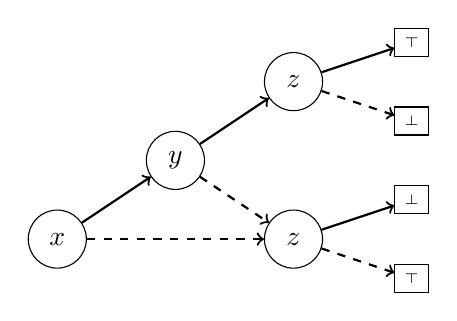
\begin{tikzpicture}
        \tikzstyle{bdd_node}       = [shape = circle,    draw = black, minimum size=21pt]
        \tikzstyle{bdd_leaf}       = [shape = rectangle, draw = black, minimum size=8pt]

        \node[bdd_node] at (0.0, 0.0) (n1) {$x$};

        \node[bdd_node] at (1.5, 1.0) (n2) {$y$};

        \node[bdd_node] at (3.0, 2.0) (n3) {$z$};

        \node[bdd_leaf] at (4.5, 2.5) (n3_l1) {\tiny $\top$};
        \node[bdd_leaf] at (4.5, 1.5) (n3_l2) {\tiny $\bot$};

        \node[bdd_node] at (3.0, 0.0) (n4) {$z$};
        \node[bdd_leaf] at (4.5, 0.5) (n4_l1) {\tiny $\bot$};
        \node[bdd_leaf] at (4.5,-0.5) (n4_l2) {\tiny $\top$};

        \draw[->, solid, thick]
          (n1) edge (n2)
          (n2) edge (n3)
          (n3) edge (n3_l1)
          (n4) edge (n4_l1)
        ;

        \draw[->, dashed, thick]
          (n1) edge (n4)
          (n2) edge (n4)
          (n3) edge (n3_l2)
          (n4) edge (n4_l2)
        ;
      \end{tikzpicture}

      \vspace{10pt}

      $f(x, y, z) \equiv \neg( (x \land y) \oplus z )$
    \end{column}
    \begin{column}{0.6\textwidth}
      \onslide<2->{
        Used in the context of:
        \begin{itemize}
        \item Model Checking
        \item Compilers
        \item Game Solving
        \end{itemize}
      }

      \vspace{10pt}

      \onslide<3->{
        Features of BDDs:
        \begin{itemize}
        \item (Often) Smaller than Formula/Set
        \item Operation Complexity depends on BDD Size
        \item Size depends on Variable Ordering
        \end{itemize}
      }
    \end{column}
  \end{columns}

  \onslide<4-> {
    % Astronauts picture
    {\leavevmode\makebox(0,0){\put(110,100){
          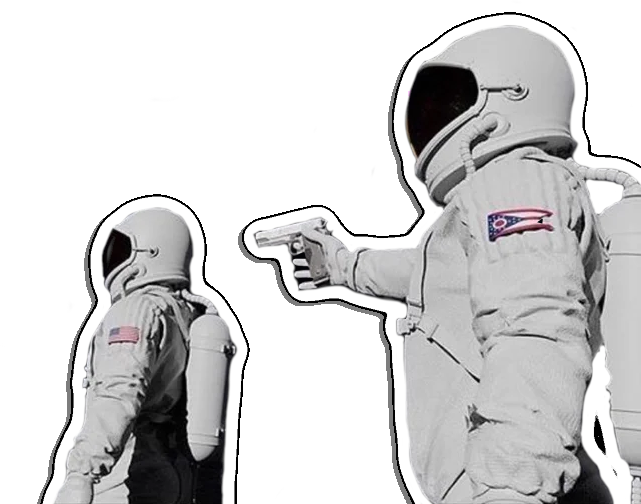
\includegraphics[width=11cm]{img/astronauts.png}

          {\put(-210,240){\fcolorbox{black}{black!20!white}{
                \large Always has been.
              }}
          }

          {\put(-350,160){\fcolorbox{black}{black!20!white}{
                \large Wait, this was about BDDs?
              }}
          }
        }
      }
    }
  }
\end{frame}

% ------------------------------------------------------------------------------------------------ %
\blankframe
% ------------------------------------------------------------------------------------------------ %

\begin{frame}[plain,noframenumbering]
  {\Large \textbf{Steffan Christ Sølvsten}}

  \begin{itemize}
  \item[\faIcon{envelope}] \mailto{soelvsten@cs.au.dk}
  \end{itemize}

  \vspace{10pt}

  {\Large \textbf{Wordrow}}
  \vspace{1pt} {\hrule width0.45\linewidth}

  \vspace{5pt}

  \begin{itemize}
  \item[\faIcon{dice}\hspace{2pt}]
    \href{http://wordrow.io}{wordrow.io}
  \item[\faIcon{code}]
    \href{http://github.com/ssoelvsten/wordrow}{github.com/ssoelvsten/wordrow}
  \end{itemize}

  \vspace{10pt}

  {\Large \textbf{Anatree}}
  \vspace{1pt} {\hrule width0.45\linewidth}

  \vspace{5pt}

  \begin{itemize}
  \item[\faIcon{code}]
    \href{http://github.com/ssoelvsten/anatree}{github.com/ssoelvsten/anatree}
  \end{itemize}

  \vspace{10pt}

  
\includegraphics[width=0.2\linewidth]{external/aulogo_uk_var2_black.eps}
\end{frame}

\end{document}